\documentclass[a4paper,12pt]{article}
\usepackage[english]{babel}
\usepackage{graphicx}
\usepackage{tikz}
\usepackage{wrapfig}
\usepackage{array}
\usepackage{color} 
\usepackage{hyperref}
\usepackage{enumitem}
\usepackage[font=small,labelfont=bf]{caption}
\hypersetup{
    colorlinks,
    citecolor=black,
    filecolor=black,
    linkcolor=black,
    urlcolor=black
}
\usepackage{changepage}

\begin{document}

\title{%
  Group Project Part 1 - Neo4j \\
  \large of Systems and Methods for Big
    and Unstructured Data Course \\(SMBUD)\\
    held by\\ Brambilla Marco\\ Tocchetti Andrea \\
  \vspace{5mm}
  \Large \textbf{Group 14}}
\author{Banfi Federico\\
  \texttt{10581441}
  \and
  Carotenuto Alessandro\\
  \texttt{10803080}
  \and
  Donati Riccardo\\
  \texttt{10669618}
  \and
  Mornatta Davide\\
  \texttt{10657647}
  \and
  Zancani Lea\\
  \texttt{10608972}}
\date{Academic year 2021/2022}
\maketitle
\begin{center}
  \includegraphics[width=4cm]{polilogo.png}\\
\end{center}
\newpage
\tableofcontents
\newpage

\section{Problem Specification}
\paragraph{}The sanitary emergency caused by the spread of the SARS-CoV-2 virus and the pandemic that has spread since 2019 has highlighted how the Big Data and the applications based on the large-scale use of these technologies can lead to concrete and effective results in a short time. Among the main examples that can be cited with regard to these there is the contact tracing, i.e. the process of attempting to identify people who have recently been in contact with someone diagnosed with an infectious disease, especially in order to treat or quarantine them. \par
The purpose of our group project is to build an information system that allows us to manage pandemic information for a given country. In order to do this we have to design, store and query a graph data structure in a NoSQL DB, by means of the graph database management software Neo4j, supporting a contact tracing app for COVID-19.
\section{Hypotesis}
\paragraph{} The way in which the database was structured and implemented is based on some hypotheses discussed in the design phase. \par Considering a typical scenario in which each person can interact either with people who live with him (family members or roommates) or with other people who go to meet voluntarily or not in a limited closed place (for example a gym, a public place, a restaurant, etc.) or in an open place located in a generic position, it was assumed that the infection can occur if during the contact between the two subjects (one of which is potentially infected) the distance between them was particularly close and if the contact duration was at least 15 minutes. In addition, to check the state of health of each individual in relation to the pandemic situation, it is essential to consider whether they have been given a vaccine and/or whether they have recently undergone a test to check for any positivity. \par
Specifically, in order to simulate the pandemic situation in the most realistic way possible and to optimally manage the available data that an information system directly connected to an app supported by the database will have to process, the following assumptions were taken into consideration:
  \begin{enumerate}[noitemsep]
    \item people can go to public places even without a green pass (therefore without a vaccine or a negative test carried out in the last 48 hours),
    \item data relating to public places are sent to the system by the manager of the public place itself,
    \item to record a greater number of relationships to be processed, while ensuring the consistency and meaningfulness of the stored data, it was decided to limit to an example study case in which the interactions present in the dataset are related to the single city of Milan and for a limited time interval, therefore:
  \begin{itemize}[noitemsep]
    \item[-] the meetings between people and the visits to public places took place within a month, in particular, to test the queries more easily, there is a specific date that expressely presents multiple recorded interactions,
    \item[-] the test and vaccine dates are all within the last 3 months,
    \item[-] all public places are located in Milan,
    \item[-] meetings between people are geolocated within the city limits
  \end{itemize}
    \item with regard to the various connections that can exist between several people and the infections that can occur within the same family, it was preferred, for design purposes, to consider the concept of "same residential unit" (i.e. residence) rather than that of "family ", since belonging to a given family unit does not necessarily imply a constant coexistence (e.g. workers who often travel for a job or off-site students) while a relationship of coexistence between several people, not necessarily related to each other, usually involves a close and inevitable contact,
    \item concerning to meetings between two or more people, it was assumed that any contact tracing devices/ apps interact with the system, communicating this information for each meeting: person1, person2, time at which the contact took place, geographical point in where the contact took place,
    \item a person is considered infected from the moment he undergoes a test and receives a positive result until he takes another test again but it is negative,
    \item in the event that a person undergoes a test and receives a positive result, all people met in the 15 days prior to the test will receive an alert notification on the app ensuring the privacy of the infected person is safeguarded,
    \item the possibility has also been envisaged in which a person already vaccinated may still be infected, in line with the cases that actually occurred
  \end{enumerate}
\clearpage
\section{ER diagram}
\paragraph{}
	\begin{center}
 		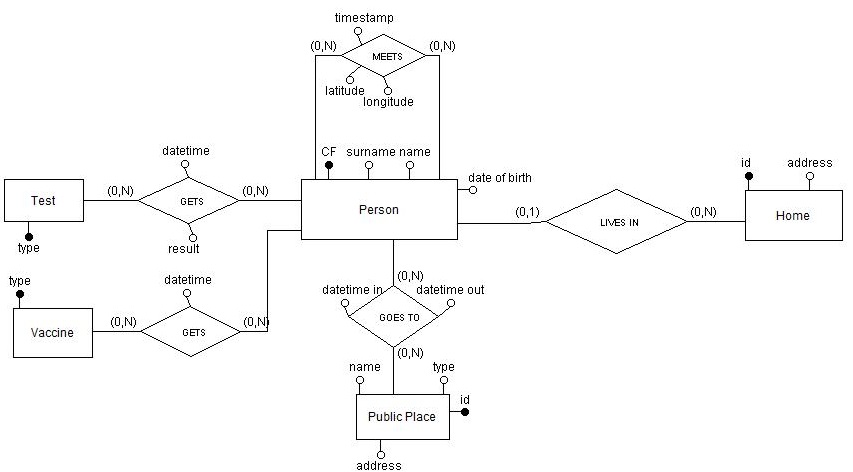
\includegraphics[width = 10 cm]{ER_diagram.jpg}
		\captionof{figure}{E-R Diagram}
	\end{center}
\par Starting from the considerations previously exposed regarding the implementation hypotheses, we have drawn an E-R diagram which includes 5 different entities and 3 many-to-many relationships described below in the logical model: \par
  \begin{itemize}[noitemsep]
   	\item[-]	\textbf{Person}(\underline{CF}, Name, Surname, DateOfBirth)
	\item[-]	\textbf{Vaccine}\underline{(Type})
	\item[-]	\textbf{Test}(\underline{Type})
	\item[-]	\textbf{PublicPlace}(\underline{ID}, Name, Type, Address)
	\item[-]	\textbf{Home}(\underline{ID}, Address)
	\item[-]	\textbf{Meets}(\underline{Person.CF}, \underline{Person.CF}, Latitude, Longitude, Timestamp)
	\item[-]	\textbf{GetsTest}(\underline{Person.CF}, \underline{Test.Type}, Datetime, Result)
	\item[-]	\textbf{GetsVaccine}(\underline{Person.CF}, \underline{Vaccine.Type}, Datetime)
	\item[-]	\textbf{GoesTo}(\underline{Person.CF}, \underline{PublicPlace.ID}, DatetimeIn, DatetimeOut)
  \end{itemize} \par
The \textbf{Person} entity describes every possible individual with his own personal data, \textbf{Test} and \textbf{Vaccine} concern the Covid-related information of each one. The \textbf{Home} entity allow us to keep track of all the people who share the same housing unit, while with \textbf{PublicPlace} it is possible to check who was in a specific place identified by an address from a certain time until it went out. Finally, the \textbf{Meets} relationship is used to keep track of all the people that everyone can meet during the day by recording with whom the meeting took place, when and where based on geographical coordinates, storing data only if the meeting duration was at least 15 minutes accordingly with the hypotheses specified before.
\section{Dataset description}
\paragraph{} One of the most critical parts of working with Big Data is managing large amounts of data collected in large datasets. To test and simulate the use of the database for contact tracing activities, some sample datasets were generated, saved in .csv format and imported into Neo4j through the command: \texttt{LOAD CSV FROM "file: ///file.csv" AS ...}. \par
Each dataset is divided into various fields that trace the structure of the tables expressed in the ER model, each one was generated randomly through python scripts and to experiment and perform at best the possible tests on the queries and commands that can be executed thanks to Neo4j the number of entries foreseen for each dataset is in the order of magnitude of the hundreds, as a whole, starting exclusively from the data loaded from the datasets, the database provides:
\begin{center}
\begin{tabular}{|l|l|l|l|}
\hline
Homes & 101 & Residence Relationship & 300 \\
\hline
People & 300 & Meetings & 726 \\
\hline
Public Places & 20 & Public Places Visits & 600 \\
\hline
Vaccine Types & 4 & Vaccinations & 526 \\
\hline
Test Types & 2 & Tests & 450\\
\hline
\textbf{TOTAL NODES} & \textbf{427} & \textbf{TOTAL RELATIONSHIPS} & \textbf{2602}\\
\hline
\end{tabular}
\end{center}

\section{Queries and Commands}
\paragraph{} The correct functioning of the information system involves the implementation of some essential commands and queries for the database in order to properly support the app and to ensure the right execution of searches among the data available for statistical or practical purposes. \par
The main commands that have been developed are those that are used to populate the database in the initialization phase starting from the previously generated datasets (e.g. load houses, people and associate each one with their residence, load public places and visits made by each one, upload meetings between more people) and to generate the entities and relationships previously described, such as vaccines and tests and their connection to various people. In addition, other more specific commands have been developed to manage typical situations or to modify the database data, such as: updating the address of a person who moves, updating the name of a public place by the manager, creating a new meeting between two people or a visit to a public place, deleting all records relating to public places that date back more than a year ago, etc. \par
Regarding the queries, the main ones considered concern a series of analyzes that can be useful both for statistical purposes in the field of data science to analyze the pandemic situation of the moment and to produce effective predictive models and/or for more concrete purposes related to human activities and immediate management of the consequences of the pandemic on daily life. The most relevant queries examined are:
  \begin{itemize}[noitemsep]
   \item[-] find how many people went without greenpass in a public place, slight variation: how many people are currently without greenpass,
    \item[-] find the family/cohabitants of an individual and check if there are infected subjects among them,
    \item[-] find the people met in a given period of time or after a given event (e.g. positive result of a Covid-test) and then generate a graph of the meetings with the people met from that moment onwards,
    \item[-] find who has been vaccinated in a given time range to perform a sort of statistical analysis on the displayed data relating to vaccinated citizens, checking which of them has the greenpass (therefore the vaccine or test) in proportion to the total population depending on the age range,
    \item[-] find who came into contact with an infected person 15 days before the last positive test, slight variation: find who went to the same public place at overlapping times as an infected person starting 15 days before the positive test
  \end{itemize}
\section{UI description}
\paragraph{}provide some screenshots and describe how your application works and which functionalities it implements
\section{User Guide} 
\paragraph{} describe step by step how could we run your application, remember to provide all the different tools and libraries to run it
\section{References and Sources(IF NEEDED)}
\paragraph{}if there are sources you used that are worth mentioning
\end{document}
